\subsection{Brain Module} Brain module is the core functional part of this thesis. It is named as Brain since it refers to the anatomical brain that plays the vital role of the human life in learning, classifying, predicting and decision making. 

Brain module is composed of 3 components which are UDP Client, Brain (Gesture Recognition Pipeline) and WebSocket Server. Flowchart \ref{fg:brain:flow} shows the data flow of this module where the user is asked to select Prediction or Training or Hand Viewer mode, when the program is started. It creates a thread and runs a loop on the main thread depending on the selection: 
\begin{itemize}
	\item UDP Client thread - Asynchronously receiving data from HRI module and thread is always running. 
	\item Prediction or Training of Hand Viewer on main program thread - Loop in the main thread run always and check if the Brain module is in prediction or training mode. If loop is interrupted, then the thread is exited and finally program is closed. 
\end{itemize}

\begin{figure}
	[h] \centering 
	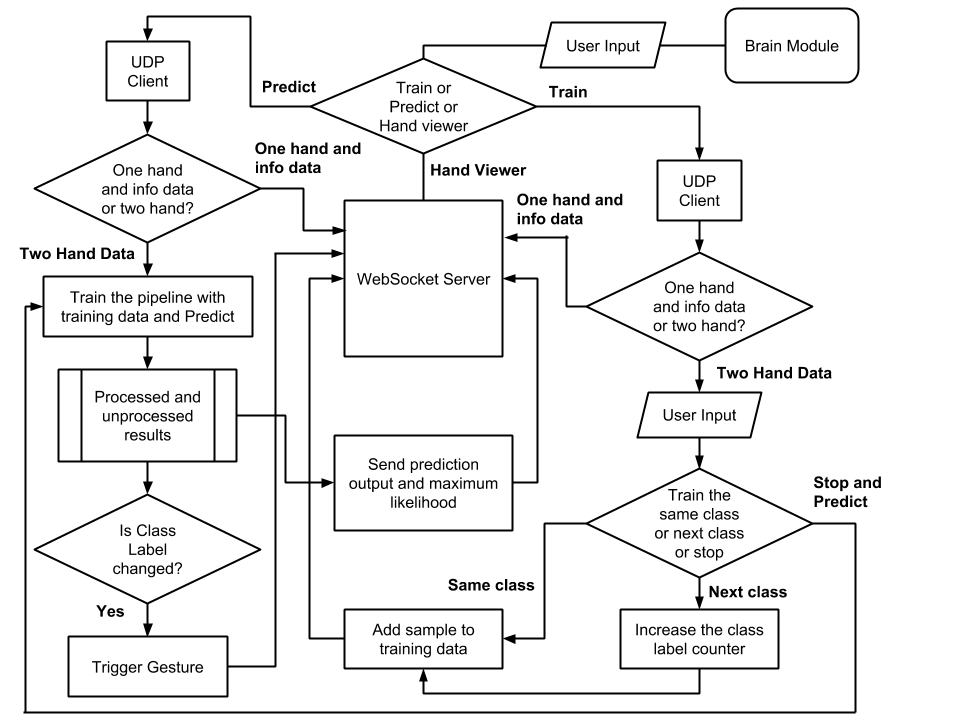
\includegraphics[height=115mm]{figures/content/brain-flow.png} \caption{Brain Module Control Flow} \label{fg:brain:flow} 
\end{figure}


\subsubsection{UDP Client} Brain module receives processed information such as joint positions, detection of focus gestures and info messages from the HRI module as UDP stream of JSON strings via WLAN. Like the UDP Server built inside HRI module, this is also an asynchronous client that starts at port 5006 and connects to the server by resolving the \textit{serverHostName} and port number from the common configuration file. Once it is connected, it receives the data from HRI module, when it is started tracking a hand or skeleton and asynchronously calls the callback handler.

Since data is transmitted as JSON strings, it has to be parsed and relevant informations must be extracted. For this purpose RapidJSON parser is used. Data flow of Brain module is mainly handled in the callback handler of UDP client because it acts as a source of input. Whenever there is a new data arrived, this asynchronous callback handler is called and it does the following tasks as shown in the flowchart \ref{fg:brain:flow} : 
\begin{itemize}
	\item Extract only newly received data from the buffer by trimming the JSON 
	\item Parse the trimmed JSON to populate hand data vectors. 
	\item If focus gesture or info messages or only one hand data is received, send it via WebSocket to the clients 
	\item Check if the module is Prediction or Training or Hand Viewer mode 
	\item In the prediction mode : 
	\begin{itemize}
		\item If the positions of both hands are received, predict the class label 
		\item Add predicted class label and maximum likelihood to the sample, and send it via WebSocket 
		\item If there is a class label not than 0, then send the respective gesture name via WebSocket 
	\end{itemize}
	\item If it is in the training mode and both hands are received, then add them to the training data 
	\item If it is in the hand viewer mode, just forward all the data to the clients via WebSocket 
\end{itemize}

\subsubsection{Brain} This is the core component of Brain module that plays a vital role in training, classifying and predicting the hand gestures. As described in the section \ref{sec:grt}, this component is based on the gesture recognition pipeline provided by Gesture Recognition Toolkit (GRT).

Flowchart \ref{fg:brain:flow} shows various tasks involved in training and predicting phase of this module. However, GRT pipeline must be configured and customized in order to be a productive gesture recognition system.

\paragraph*{Classifier} Adaptive Naive Bayes Classifier (ANBC) is used in this thesis as described in the section \ref{sec:anbc}. Training data for the same gesture will vary in range from person to person and position to position. Therefore the classifier is enabled for Min-Max scaling that is basically a normalization by rescaling the values between 0 to 1. This is done by calling \textit{enableScaling(true)} function of the classifier.

\paragraph*{Null Rejection} Enabling the scaling with ANBC will classify every input samples to belong to any of the class and thereby, do not have the ability to detect non-gestures. To avoid this catastrophe GRT offers Null Rejection features to the algorithms, by this function \textit{enableNullRejection(true)} and also provides a function to set how big the rejection region should be, by \textit{setNullRejectionCoeff(1)}.

\paragraph*{Post Processing} As discussed in the section \ref{sec:grt}, prediction output must be post processed in order to avoid false prediction spikes. Therefore, class label filter is added to the pipeline by with this function \textit{ClassLabelFilter(30,60)}. Minimum count is set to 30 with the buffer size of 60 for the reason that the user must gesticulate for minimum of one second since depth camera produces 30 frames per second. Additionally \textit{ClassLabelChangeFilter()} is added so that there is only one output of the predicted class label, when there is a change in the gesture and all other time it outputs 0, that is reserved for non-gesture.

\paragraph*{Training Data} We used \textit{ClassificationData} data structure of GRT to collect training data of static gestures. It must be initialized with number of dimensions the samples will be. In our thesis we modeled hand gestures with two hand positions in 3 dimensional Cartesian coordinates, therefore training dataset has 6 dimensions. As described in the section \ref{sec:grt}, GRT enables us to execute various operations on the training data such as recording, labeling, partitioning and testing. 

\paragraph*{Training} When Brain is set to training mode, it starts the \textit{TrainingDataRecordingTimer}. We have configured 20 seconds recording time and 15 seconds preparation time. Preparation time helps the trainer to go in front of depth camera and stay in the pose of the gesture that is going to be recorded. Furthermore, It initializes the Class Label to 1 and it will be increased by one for other classes. Class Label can not be assigned to 0 because GRT reserves it for non-gestures. If positions of left and right hand are received from the HRI module, Brain starts to add the samples with the chosen Class Label to the training dataset till the timer is in recording mode and simultaneously it sends to received samples via WebSocket to the clients to visualize. When the recording timer is stopped, Brain requests the trainer to choose any of the following options : 
\begin{itemize}
	\item Train the same class again - New samples will be added to the training dataset for same Class Label. 
	\item Train the next class - Class Label is increased by one and new samples are added. 
	\item Stop training and go to prediction mode - Saves the training dataset to a file named as \textit{hri-training-dataset.txt} and trains the pipeline and goes into prediction mode 
\end{itemize}

\paragraph*{Prediction} When Brain is set to prediction mode, first thing it does, is loading the training labeled classification data and train the pipeline to create models for each gesture. Second step is to look for any specific pipeline configuration such as classifier and pre/post processing modules. Such configurations can also be loaded into pipeline as GRT pipeline files. This feature of GRT offers us an opportunity to run the gesture recognition application using dynamic configurations. Once Brain starts to receive input samples via UDP, it feeds it to the pipeline to predict. Finally, the prediction results such as predicted class label, maximum likelihood, class distances and weights are returned by the pipeline. Flexible GRT pipeline provides many more features such as post-processed and unprocessed prediction results. Therefore, the prediction results for every input sample can be obtained. The post-processed result will allow Brain to send the detected gesture only once, even if the user is continuously gesticulating the same gesture. 

\subsubsection{WebSocket Server} \textit{WebSocketServer} class is developed using websocketpp C++ library that basically uses BOOST libraries. It is a simple implementation of WebSocket server that listens to the port number 5008. The port number can be configured dynamically by loading the common configuration file. WebSocket class is initialized by UDP Client class and keeps the server running in a separate thread. Once clients such as CC module and Command module are connected, it stores the endpoint connection handlers of them for later communication. 
